\chapter{Background}\label{sec:background}

    % \begin{blockquote}
    %     \paragraph{Intent:} General background information needed to follow the terms and methods used in this thesis. 
                
    %     Structure:
    %     \begin{description}
    %         \item[1. Parameter tuning] Parameter tuning of a black-box
    %             \begin{enumerate}
    %                 \item $f(Parameter) = Objective$ 
    %                 \item Goal is optimize $f$
    %                 \item Problem: Optimization of multiple objectives
    %             \end{enumerate}
    %         \item[2. Multi-objective optimization] General definition. Pareto front and None-dominated solution
    %             \begin{enumerate}
    %                 \item What is a multi-objective solution?
    %                 \item How to compare solutions? $\rightarrow$ Types of metrics
    %                 \item How to solve? $\rightarrow$ Scalarizing, MOEA, Random
    %                 \item Problem: Reduce evaluations $\rightarrow$ Surrogate optimization, MBMO
    %             \end{enumerate}
    %         \item[3. Surrogate optimization] Approach for reducing evaluation count
    %             \begin{enumerate}
    %                 \item Intro. Cons and Pons
    %                 \item Types of a surrogate model in a MO-problem (Model of scalarization, MO-model, Replicated MO-model, Compositional MO-model). Taxonomy
    %                 \item Surrogate assistance for MO parameter tuning $\rightarrow$ Reusable/scalable components for optimization $\rightarrow$ Problem: Scalability of a surrogate model.                  
    %                 \item Surrogate model is domain-specific $\rightarrow$ Analyze multiple surrogates $\rightarrow$ Surrogate portfolio [RQ1 \ref{RQ1}]
    %                 \item Sampling plan. Build a surrogate model. Quality of prediction depends on the accuracy of a surrogate model  $\rightarrow$ Accuracy depends on a sample size $\rightarrow$ Sample size depends on surface type $\rightarrow$ Problem: Sample size is static. [RQ2 \ref{RQ2}]
    %                 \item Surrogates and MOEA are hard scalable 
    %             \end{enumerate}
    %         \item[4. Scope of work] Starting point of thesis
    %             \begin{enumerate}
    %                 \item Problem: Expensive black-box with multiple objectives
    %                 \item Constraint: Evaluation budget
    %                 \item Goal: Set of MO solutions closed to Pareto-front $\rightarrow$ 1.$Max$ Hypervolume, 2.$Min$ Points-Space, 3.$Max$ \% of None-Dominated points 
    %                 \item Solution approach: Surrogate model(s) with MOEA
    %             \end{enumerate}
    %     \end{description}
    % \end{blockquote}

    This chapter presents general background information needed to follow the terms and methods used in this thesis. 

    % --------------------------------------------------------------------------------------------
    % ------------------------------------------------        Parameter tuning
    % --------------------------------------------------------------------------------------------
    \section{Parameter tuning}
        We start by introducing a parameter tuning problem. We consider a objective function as a black-box $f : \mathbb{S} \rightarrow \mathbb{R}$ with parameter and objective spaces (Fig. \ref{fig:spaces}). All feasible combinations of parameters define a parameter space which is intended to be a function input $\mathbb{S}$, and therefore all possible function outputs are defined as an objective space or $f(x), x \in \mathbb{S}$. The minimization of the fitness function could be defined as follows:

                \begin{equation} \label{eq:arg_min}
                    x^* = \underset{x \in \mathbb{S}}{\arg\min} f(x)
                \end{equation}

        % --- spaces
        \begin{figure}
            \centering 
            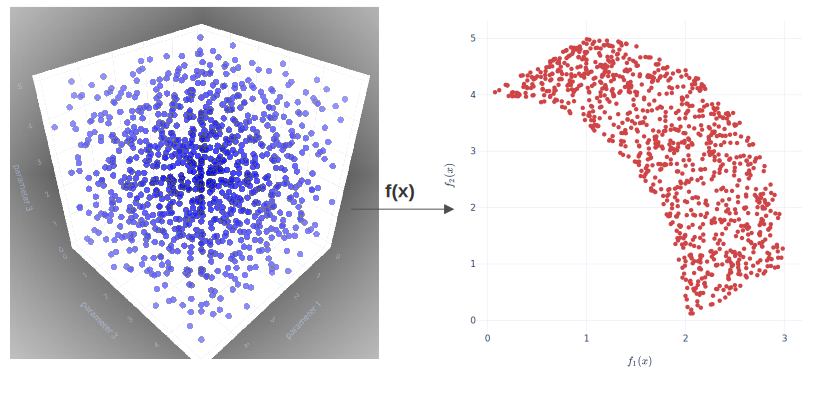
\includegraphics[width=0.8\textwidth]{content/images/utility/spaces}
            \caption[Example with a uniformly distributed points in the parameter space (left) with the corresponding values of these parameters in the objective space]{Example with a uniformly distributed points in the parameter space (left) with the corresponding values of these parameters in the objective space (right). As can be noted from the results, the optimization of both objectives ($f1$, $f2$) is contradictive.} 
            \label{fig:spaces} 
        \end{figure}

        The mapping of all points from the parameter space to the points in the objective space is called a fitness landscape. The task of the parameter tuning as an optimization task is to find optimal points on this surface. Depending on the type of a landscape, the optimization search often yields qualitatively different behaviour.
        The single criterion in the parameter tuning might not be sufficient to characterize the behaviour of the configuration space correctly. Therefore, multiple criteria have to be considered. Typical examples of such objectives are to enhance accuracy and performance or minimize runtime, error rate and energy. The parameter tuning process should improve the objectives of those in which none of the objectives can be improved without affecting another objective. By default, we consider minimization for all objectives. 
        % !Typical examples - By default
        In this thesis, we are following the next properties of the parameter tuning:
        \begin{itemize}
            \item Evaluation is expensive
            \item Black-box function and number of evaluated results are unknown
            \item Multi-objectivity with global minimization
        \end{itemize}

        There is a demand on the method which can explore the search space with limited evaluation budget. 
    

    % --------------------------------------------------------------------------------------------
    % ------------------------------------------------        Multi-objective       -------------
    % --------------------------------------------------------------------------------------------
    \section{Multi-objective optimization}
        Common parameter tuning problems require a simultaneous optimization of multiple, usually contradictive objectives $f = (f_1(x), \ldots, f_k(x))$. Multi-objective optimization deals with such conflicting objectives. It provides a mathematical algorithm to obtain an optimal design state which accommodates the various criteria demanded by the situation. Objectives are being improved simultaneously and gradually.

        The solution of the multi-objective problem is a group of points which are placed on a Pareto front; i.e. the subset of solutions which are not worse than any other but better on at least one goal \cite{KrallMD15}. The solution called a Pareto optimal if any other solution does not dominate it. For example (Fig. \ref{fig:dominated}) a solution $A \in \mathbb{S}$ is said to dominate another solution $B \in \mathbb{S}$ , denoted $A \preceq B$ if $f_i(A)<=f_i(B)$ for all $i=1, \ldots ,k$ and $f_i(A)<f_i(B)$ for at least one $i \in \{1, \ldots k\}$. All points on the Pareto frontier are not-dominated by any other point in the objective space \cite{Kaisa0021267}.  

        Awareness of the Pareto front allows appropriate decisions and the importance of the criteria to be visualized. For the multi-objective problem we consider the solution as points from the parameter space which lead to non-dominated results in the objective space. The improvement of the solution means that a set of points corresponds better with the real Pareto-front.

        % ==== dominated
        \begin{figure}
            \centering 
            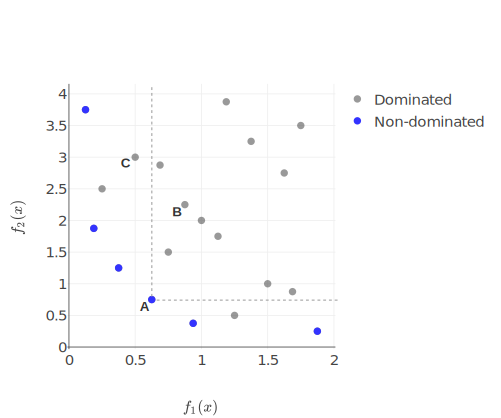
\includegraphics[width=10cm]{content/images/ndom}
            \caption[Non-dominated points]{Example of non-dominated points. Point A dominates all points in the internal sector where B is located. Concerning the point A, the point C is not dominant because it has better value in $f_1$} 
            \label{fig:dominated} 
        \end{figure}

        % There exist various techniques to solve multi-objective problems: 
        % % --- Grid search and Random search
        % \subsubsection{Grid search and Random search} 
        % The main advantage of these algorithms lay on their simplicity. Grid search evenly covers a search space but requires functions evaluations growing exponentially with increasing dimensionality of configuration space. Random search works better when some parameters are more significant than others but still require more function evaluations to find optimal regions.

        % These methods are a good baseline to compare more complex techniques. 

        % % --- Heuristics and Metaheuristic
        % \subsubsection{Heuristics and Metaheuristic}
        % (Simulated annealing, Evolutionary algorithm) a family of non-exact algorithms including evolutionary algorithms and swarm intelligence methods. These methods aim at generating approximately optimal solutions in a single run. It also could operate with sets of solutions, being outcomes of multiple objectives.

        % % --- Sequential design
        % \subsubsection{Sequential Model-Based Optimization}
        % (Bayesian optimization, Evolutionary algorithm) Bayesian methods differ from random or grid search in that they use past evaluation results to extrapolate and choose the following values to evaluate. Limit expensive evaluations of the objective function by choosing the following input values based on those that have done well in the past.
        % limit expensive evaluations of the objective function by choosing the next input values based on those that have done well in the past.

    % ------------------------------------------------        Metrics       -------------
        \subsection{Metrics for multi-objective solution}
            In a single-objective optimization the quality of a given solution is trivial to quantify. When we consider a solution of a multi-objective problem as a Pareto-optimal approximation, the comparison of these solutions is also a multi-objective task.
            The question of picking metrics for evaluation is essential for comparison of approximated solutions and for selection of the next appropriate set of configurations.

            According to \cite{ZitzlerDT00}, a Pareto front approximation should satisfy the following criteria:
            \begin{itemize}
                \item The distance between Pareto front and its approximation should be minimized.
                \item A wide distribution of non-dominated points is desirable.
                \item The range of the approximated front should be maximized, i.e., for each objective, a wide range of values should be covered by the non-dominated points.
            \end{itemize}

            The metrics for performance indicators were partitioned into four groups according to their properties \cite{Audet2018PerformanceII}: 
            \begin{itemize}
                \item \textit{Cardinality.} Estimation of number of non-dominated points.
                \item \textit{Convergence.} Estimation of closeness of a set of non-dominated points to the Pareto front in the objective space.
                \item \textit{Distribution and spread indicators.}  Measurement of the points distributed on the Pareto front approximation or of there spreadness in extreme points of the Pareto front.
                \item \textit{Convergence and distribution indicators.} Capture of both: the properties of convergence and distribution.
            \end{itemize}

            According to \cite{CustodioMVV11} the spread metrics try to measure the areas achieved in a computed Pareto front approximation. This type of metrics is not very useful for comparison of algorithms or for evaluation of optimization convergence because spreadness is not related to improvement the objectives. However, they could be useful for a more detailed analysis of the optimization process or for composing Pareto frontier from several solutions.

            The goal of the multi-objective optimization is to obtain an approximated solution set with the reference to the Pareto front, including the following subgoals:
            \begin{itemize}
                \item All solution sets are as close as possible to the Pareto front.
                \item All solution sets are as diverse as possible in the objective space.
                \item The proportion of the solution set to the evaluated set is as large as possible. 
                \item Evaluate as few solutions as feasible.
            \end{itemize}

            For multi-objective optimization, an algorithm should produce a set of solutions which provide the optimal trade-off between the considered optimization objectives. Therefore, the performance comparison of \gls{moo} algorithms is based on their Pareto sets. In this study, four well-known metrics are used to quantify the performance of the algorithms.
            \begin{itemize}
                \item \textbf{Hypervolume (HV).}\cite{ZitzlerDT00} \textit{Convergence and distribution indicator.}
                This metric represents the volume of the objective space which is covered by the individuals of non-dominated solutions which belong to the Pareto front (Figure \ref{fig:hypervolume}). Two points delimit the volume: one point represents the reference point $r$ ($r \in R^m$) which is defined as the worst solution inside the objective space; another one represents the point which represents Pareto approximation $S$, for all $z \in S, z \prec r$. The hypervolume metric is defined as follows:

                    \[HV(S,r) = \lambda_m(\bigcup\limits_{z \in S} [z;r])\]

                where $\lambda_m$ is m-dimensional Lebesgue measure.    
                Calculating the hypervolume indicator is a computationally expensive task. Furthermore, in case of a small number of dimensions and a low number of points, there are currently no known algorithms which might return the results fast enough for the use in most algorithms due to computational complexity which is 
                $\mathcal{O}(|S|^{\frac{m}{2}}\log{|S|}) $ \cite{BeumeFLPV09}.
                \item \textbf{Non-dominated Ratio (NDR).} \textit{Cardinality.} This metric is a ratio between the number of non-dominated points and the total number of the evaluated points.  Higher values are preferred to lower ones.
                \item \textbf{Spacing \cite{Schott1995FaultTD}.} \textit{Distribution and spread.} Description of the distribution of Pareto points. As a wide range of similar metrics which are based on the distance to the nearest neighbour, spacing does not cover the holes in Pareto frontier and might compute the distribution in solution clusters.
                \item \textbf{$\Upsilon$-metric (p-distance)}\cite{Martens13} \textit{Convergence} This metric is an average distance of a set of points in relation to the Pareto front. $\Upsilon$-metric is defined by

                    \[\Upsilon(S) = \frac{1}{|S|}\sum_{z\in S}g(z)-g(x^*)\]
                where $g$ is a distance function and $x^*$ Pareto-optimal decision vector.
                The lower the $\Upsilon (S)$, the closer the solutions of S are to the solutions of the Pareto-front. 
                
            \end{itemize}

            % -------------------------------------- Hypervolume
            \begin{figure}
                \centering
                \begin{subfigure}{\textwidth}
                    \begin{subfigure}{0.45\textwidth}
                        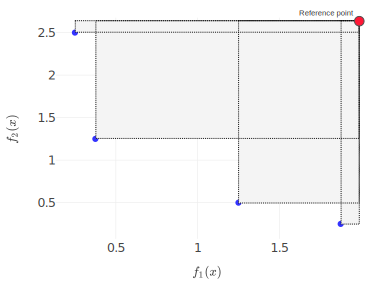
\includegraphics[width=\textwidth]{content/images/utility/hypervolume}
                        \caption{Higher hypervolume values may correspond to a better distribution of solutions or closeness to the Pareto frontier.}
                        \label{fig:hypervolume_basic}
                    \end{subfigure} 
                    \begin{subfigure}{0.45\textwidth}
                        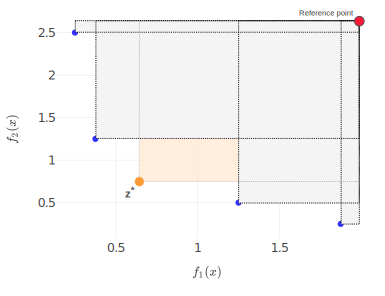
\includegraphics[width=\textwidth]{content/images/utility/hypervolume_impr}
                        \caption{Example of hypervolume improvement with a new non-dominated point z* in the solution set.}
                        \label{fig:hypervolume_impr}
                    \end{subfigure} 
                \end{subfigure} 

                \caption[Visualization of hypervolume metric for a bi-objective set of non-dominated points]{Visualization of hypervolume metric for a bi-objective set of non-dominated points.}
                \label{fig:hypervolume}    
            \end{figure}
 
    % ------------------------------------------------        Solving methods       -------------
        \subsection{Solving methods}
            Finding a Pareto-optimal set is often impractical and might be computationally expensive. Therefore, many stochastic search strategies have been developed such as: evolutionary algorithms, tabu search, simulated annealing and ant colony optimization. These algorithms usually do not ensure to find ideal trade-offs but try to gain a satisfying approximation.
            In this thesis, under the Pareto-optimal front, we mean an optimal solution to the problem. All points on the Pareto-frontier are none-dominated, but not all none-dominated points are Pareto-optimal. There are several basic approaches which provide information how from non-dominated points move forward to Pareto-optimal solution.
            %!!! information how from non-dominated

            % ----------------      Scalarizing       
            \subsubsection{Scalarization}
                Scalarizing approach is a popular technique for creating a single-objective \textit{parameterized} problem with the composite criteria from multiple objectives. The main advantage of the scalarization is the possibility to use a broad range of single-objective technics to this composite function. After optimization one Pareto-optimal solution is obtained, which depends on the initial scalarization parameters. The weighted-sum method is a well-known type of scalarizing technic. This approach concatenates the objectives into a single criterion by using weighted sum factors. There are difficulties in selecting proper weights, especially when there is no correlation in the prior knowledge among objectives \cite{ChughScal2019, DerbelBLV14}. 

                Some scalarizing technics try to improve the exploration of the parameter space by assigning more "intelligent" aggregation to objectives. Such solutions might be fragile. They change dramatically with a modification of algorithm parameters. Moreover, the weighting method can not provide a solution among underparts of the Pareto surface due to the "duality gap" for not convex cases. This means the replacement of non-convex original function to convex closure which missed non-convex parts of the initial landscape. Furthermore, some of the scalarizing algorithms are very sensitive to the number of objectives. Analysis of the fitness landscape with different scalarizing techniques might be helpful in the optimization for solving expensive \gls{mop} \cite{ChughScal2019}.

                % For example, if we want to reach the point in the middle of two other points in Pareto frontier, we hardly get a peek of the Pareto surface, as long as the well-known simplex method is used. This implies that depending on the structure of the problem. The linearly weighted sum can not necessarily provide a solution as DM desires. \cite{Nakayama05}. Moreover, the weighting method can not provide a solution among underparts of the Pareto surface due to the “duality gap” for not convex cases. 

                % ? Scalable algorithms that convert multi-objective to single-objective problem solve that not accurate enough(Scalarizing). Also, this approach suitable for a limited type of problem. Moreover, there are important lot of parameters that significant influence on algorithm performance.

            % --------------------      MOEA
            \subsubsection{Multi-Objective Evolutionary Algorithms}
            An evolutionary algorithm forms a class of heuristic search methods which simulate the process of a natural evolution. The evolutionary algorithm is determined by the two basic principles: selection and variation \cite{TutMOEABrockhoff}. While selection reflects competition for reproduction and resources among individuals, the other principle, variation, imitates the natural ability to produce new individuals through recombination and mutation. 
            The evolutionary algorithms are suitable for problems, including multiple conflicting objectives and large and complicated search spaces \cite{Andersson00asurvey, RamirezRV19}. Evolutionary optimizers explore populations of candidate solutions in each generation. A mutator can make changes in the current population. A select operator then picks the best mutants, which are then combined in some way to become a new population in the next iteration. However, \gls{ea} still needs many evaluations of the black box system to solve the common multi-objective problem. This problem is crucial for the reason that most multi-criteria problems are expensive to estimate. This massive evaluation budget makes \gls{ea}s infeasible for costly and multi-objective problems.  


    % --------------------------------------------------------------------------------------------
    % ------------------------------------------        Surrogate optimization       -------------
    % --------------------------------------------------------------------------------------------
    \section{Surrogate optimization} 
        Many expensive optimization problems have a practical limitation on the number of possible estimations which standard optimization approaches spend very quickly. To get around this drawback, approximation models or surrogate models are often used. This technique is essential to reduce real evaluations by building a regression function based on already evaluated design points.
        The potential of the appliance of the surrogates is based on the generalization of the all search space and fast navigations there. This advantage should outperform disadvantage in time required to build this approximation. In classical model-based optimization, a single surrogate-model provides a hypothesis on the relation between parameter and objective spaces. The approximation of the solution becomes faster than the real evaluation, so the whole optimization process is accelerated. However, some extra time is needed to build and update the surrogate model during the optimization process. The surrogate model is used to find the probable good candidates or to drop the low-quality individuals even before they are exactly evaluated, thus, us to reduce the number of exact evaluations.

        In literature, the term surrogate or model-based optimization is used when during the optimization processes some solutions are not evaluated with the original function, but are approximated using a model of this function. Some of the most commonly used methods are represented by the Response Surface Method \cite{ResponseSurface}, Radial Basis Function \cite{Rasmussen2004}, Neural Network \cite{KOURAKOS201313}, Kriging \cite{Woodard00}, and Gaussian Process Modeling \cite{RasmussenN10, RasmussenW06}. Surrogates are also used to rank and filter out the offspring according to Pareto-related indicators like a hypervolume \cite{EmmerichGN06}, or a weighted sum of the objectives \cite{TaboadaBCW07}. If the model is a single-criterion, it could be expanded to a multi-objective surrogate by treating each criterion in isolation and duplicating the model for each of them \cite{Knowles06, nardi2019practical}. The surrogate model is either selected randomly or due to its popularity in the associated domain area \cite{SoftSurvey}. Thus, there are still some open challenges related to the combination of meta-models, such as a definition of a selection criterion or combination techniques. Besides, there are no guidelines for using heterogeneous compositional models for different objective functions \cite{SoftSurvey}.

        
        % -------------------------------------------------------------------------------------------------
        % ------------------------------------------------        MO in Parameter tuning       -------------
        \subsubsection{Multi-objective parameter tuning}

            The categorization of parameter tuning approaches based on the workflow of sequential model-based optimization is presented in Fig.\ref{fig:mo_param_tuning}. The optimization process begins with the initial sampling plan. At this stage, it is necessary to collect fitness results or to evaluate the first parameters which are used to build surrogate models. For an initial sampling plan, or a \gls{doe} plan, the techniques of the \gls{lhs}, the Sobol sampling or the random sampling can be used.
            
            % ===  Phases and tasks in parameter tuning with surrogates model
            \begin{figure} 
                \centering
                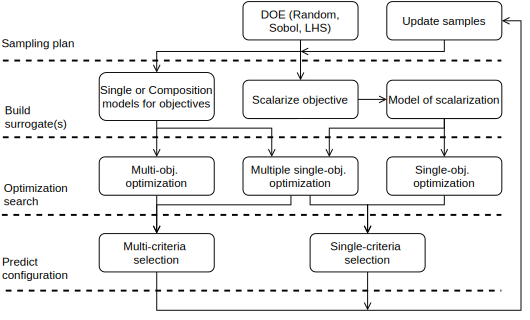
\includegraphics[width=\textwidth]{content/images/tax_mb_tuning}
                \caption[Phases and tasks within a generalized multi-objective parameter tuning]{Phases and tasks within a generalized multi-objective parameter tuning}
                \label{fig:mo_param_tuning}
            \end{figure}

            There are two approaches established to extrapolate the samples: 1) to scalarize objectives and produce a surrogate model of the this scalarization (In this case, the multi-objective problem transforms into a single-objective one); 2) to keep the original dimensionality of the problem and apply one or several models to hold and infer on the problem landscape.

            The next step is represented by the search for the optimal points within the surrogate model. At this step, the solutions which might be Pareto-optimal are found. In the predict configurations phase, sorting and selection are carried out. In the case of multicriteria selection, it is necessary to select the required number of points which are optimal for all objectives. In theory, all non-dominated points are equal regardless of the order they are chosen in. The advantage of the possible prediction of several parameters instead of a single one improves the exploration of the parameter space and parallelizing of the fitness evaluation. The required number of points allows the sample set to be estimated as sell as updated. Optimization iterations continue until the stop condition is satisfied.
    
            The variability and extensibility are essential for configurable parameter tuning, suchlike a software product line. The optimization round is consistent and universal. As shown in Fig. \ref{fig:mo_param_tuning}, the potential to reuse components in a workflow is enormous. The same single-objective models can be equally applied to various types of problems in multi-/single-objective optimization. An optimization algorithm weakly depends on the type of a surrogate model. By dynamical duplication of the surrogate model or even by the creation of several surrogate hypotheses, we aim to improve the parameter tuning to multiply criteria on-the-fly.

        % --------------------------------------------------------------------------------------------
        % ------------------------------------------------     Domain-specific Surrogate model      
        \subsection{Domain-specific problem}
        Surrogate models are domain-specific in case of intention to find the best solution with less effort. On the one hand, the surrogate model could perform well while extrapolation one class of problems and guide to the optimal solution. On the other hand, this model could be a reason for a significantly degrading result in another type of problem. That is why the authors prefer using several surrogate models and don't select one for all use cases \cite{SoftSurvey}.

        It could be an interpreter as a \Gls{nfl} in model-based optimization. If we extend this argument, then the same optimization problem in different parameter tuning iteration could be interpreted as another optimization problem. In order to reduce an effort and to increase the convergence of an algorithm, we should change the surrogate model depending on how much samples we have. 
        This leads us to the usage of a portfolio with surrogate models. On each optimization iteration, the portfolio tries to build and select several models with the best performance.  As a negative consequence, the model building introduces an additional overhead into the optimization.


        % --------------------------------------------------------------------------------------------
        % ------------------------------------------------     Build surrogate model     
        \subsection{Initial sampling set}
        Initial samples should provide maximum information to build a useful model. The overall result depends primarily on how accurate the assumption is. Invalid optimization model makes all further optimization results irrelevant. To determine it, the concept of surrogate validity is introduced, which means that the model may be used in order to find optimal solutions.

        If no valid models are gained, it is better to use the initial design than to be guided by an incorrect model. With an increasing sample size, in case of proper fitting, a better surrogate model is obtained, and the better results in optimization are reached. Moreover, the initial sample size might be too big, which is a mere waste of resources.  


    % --------------------------------------------------------------------------------------------
    % ------------------------------                    Discussion       
    \section{Discussion}
    The most methods for parameter tuning optimization are related to surrogate-based optimization. One of the main advantages of this approach is the speed of evaluation across the entire search space and possibilities to apply a broad range of optimization techniques. However, there are disadvantages, such as extra time to select and build this surrogate model. 
    It would be desirable to have a way to combine several surrogate models which are samples- and domain-dependent.


    % General classification \cite{MlakarPTF15}:
    % Within surrogate-model-based optimization algorithms, a mechanism is needed to find a balance between the exact and approximate evaluations. In evolutionary algorithms, this mechanism is called evolution control \cite{Jin05} and can be either fixed or adaptive. In fixed evolution control the number of exact function evaluations that will be performed during the optimization is known in advance. Fixed evolution control can be further divided into generation-based control, where in some generations all solutions are approximated and in the others, they are exactly evaluated \cite{DebN07}, and individual based control, where in every generation some (usually the best) solutions are exactly evaluated and others approximated \cite{Grierson1993}. In adaptive evolution control, the number of exactly evaluated solutions is not known in advance but depends on the accuracy of the model for the given problem. Adaptive evolution control can be used in one of two ways: as a part of a memetic search or to pre-select the promising individuals which are then exactly evaluated \cite{PilatN12}.

    % Direct fitness replacement and indirect fitness replacement
    % Kind of extending the search stage of MOEA with surrogate to simulate evaluation of population. It transform the problem of searching a new better population to improving general hypothesis of how and where Pareto set presented.  
